\documentclass[a4paper,11pt,twoside]{pads-thesis}


\renewcommand{\gTitle}{Thesis Title}
\renewcommand{\gAuthor}{David Benedikt Georgi}
\renewcommand{\gHeader}{Master's Thesis}
\renewcommand{\gSupervisor}{
    Supervisor}
\renewcommand{\gExaminer}{Prof. One \\ 
	Prof. Two }
\renewcommand{\gInstitution}{i9 Process and Data Science (PADS) Chair, RWTH Aachen University}
\renewcommand{\gRegDate}{YYYY-MM-DD}
\renewcommand{\gSubDate}{YYYY-MM-DD}

\begin{document}
%%% Title page
\pagenumbering{roman}

\gTitlePage
%\pagestyle{plain}
%%% TOC

%\begin{abstract}
\chapter*{Abstract} \addcontentsline{toc}{chapter}{Abstract}
The real-time prediction of business processes using event data of historical executions is a critical capability of business process monitoring systems.
Existing process prediction methods are limited in terms of the type of data they are able to utilize and the prediction tasks they can perform.
In particular, almost no technique is able to utilize text documents of natural language, which can hold process-critical information.
This work describes the design, implementation, and evaluation of a novel text-aware process prediction model based on long short-term memory (LSTM) neural networks and natural language models.
The proposed model can take categorical, numerical and textual attributes in event data into account to predict the activity and timestamp of the next event, the outcome and the cycle time of a running process instance.
Experiments show that the text-aware model is able to outperform state-of-the-art process prediction methods on simulated and real-world event logs containing textual data.
\\\\
\textbf{Keywords:} Predictive Process Monitoring, Process Mining, Text Mining, LSTM Neural Networks
%\end{abstract}

\tableofcontents

%\setcounter{page}{1}
\cleardoublepage
%%% Begin document
\pagestyle{fancy}
\pagenumbering{arabic}

\chapter{Introduction} \label{chap:intro}

\section{Motivation}

The rapid growth of data generated by large-scale information systems leads to new opportunities for  society and businesses. 
By the end of 2020, the total amount of generated data is estimated to be 44 trillion gigabytes of which 90\% has been created in the last two years \cite{datagrowth}.
In order to benefit from the massive amount of data, efficient solutions are required, that are able to extract potential value in form of models, analyses or predictions.

A remarkable subset of this data is described as \textit{event data}, which is generated by \textit{process-aware information systems}, which manage, execute and monitor business processes \cite{DBLP:journals/topnoc/Aalst09}.
With the non stopping rise of digitization of business processes, increasingly more event data becomes utilizable, thus the potential value of this data is exploding.

The scientific engagement aiming to discover, analyze and improve real processes based on event data led to \textit{process mining}. Process mining bridges the gab between the data-driven characteristic of data science and the process-centric view of process science \cite{DBLP:books/sp/Aalst16}.
The ongoing success of progress mining in research has been transferred to businesses, that successfully offer or utilize this technology.
Celonis, which is often considered as one of the biggest commercial providers of process mining, has been valued 2.5 billion dollar only 9 years after the company was founded \cite{celonis}.

Modern process mining software tends to focus on continuous monitoring and analysis of business processes, in contrast to traditional offline and project-based approaches, that are not integrated with the remaining IT infrastructure of a company.
The integrated and continuous application of process mining is realized by a \textit{business process monitoring system}, which are a key success factor for many organizations, since they allow to understand and supervise all processes of a company in real-time during the execution of the processes.
The core idea of this approach is to automate process mining and keep a persistent data connecting between the information system and the monitoring system, that provides the analytical capabilities.
Figure \ref{fig:process-monitoring} visualizes such an infrastructure and the connection between the systems and the internal and external process stakeholders.

\begin{figure}[htbp!]
	\centering
	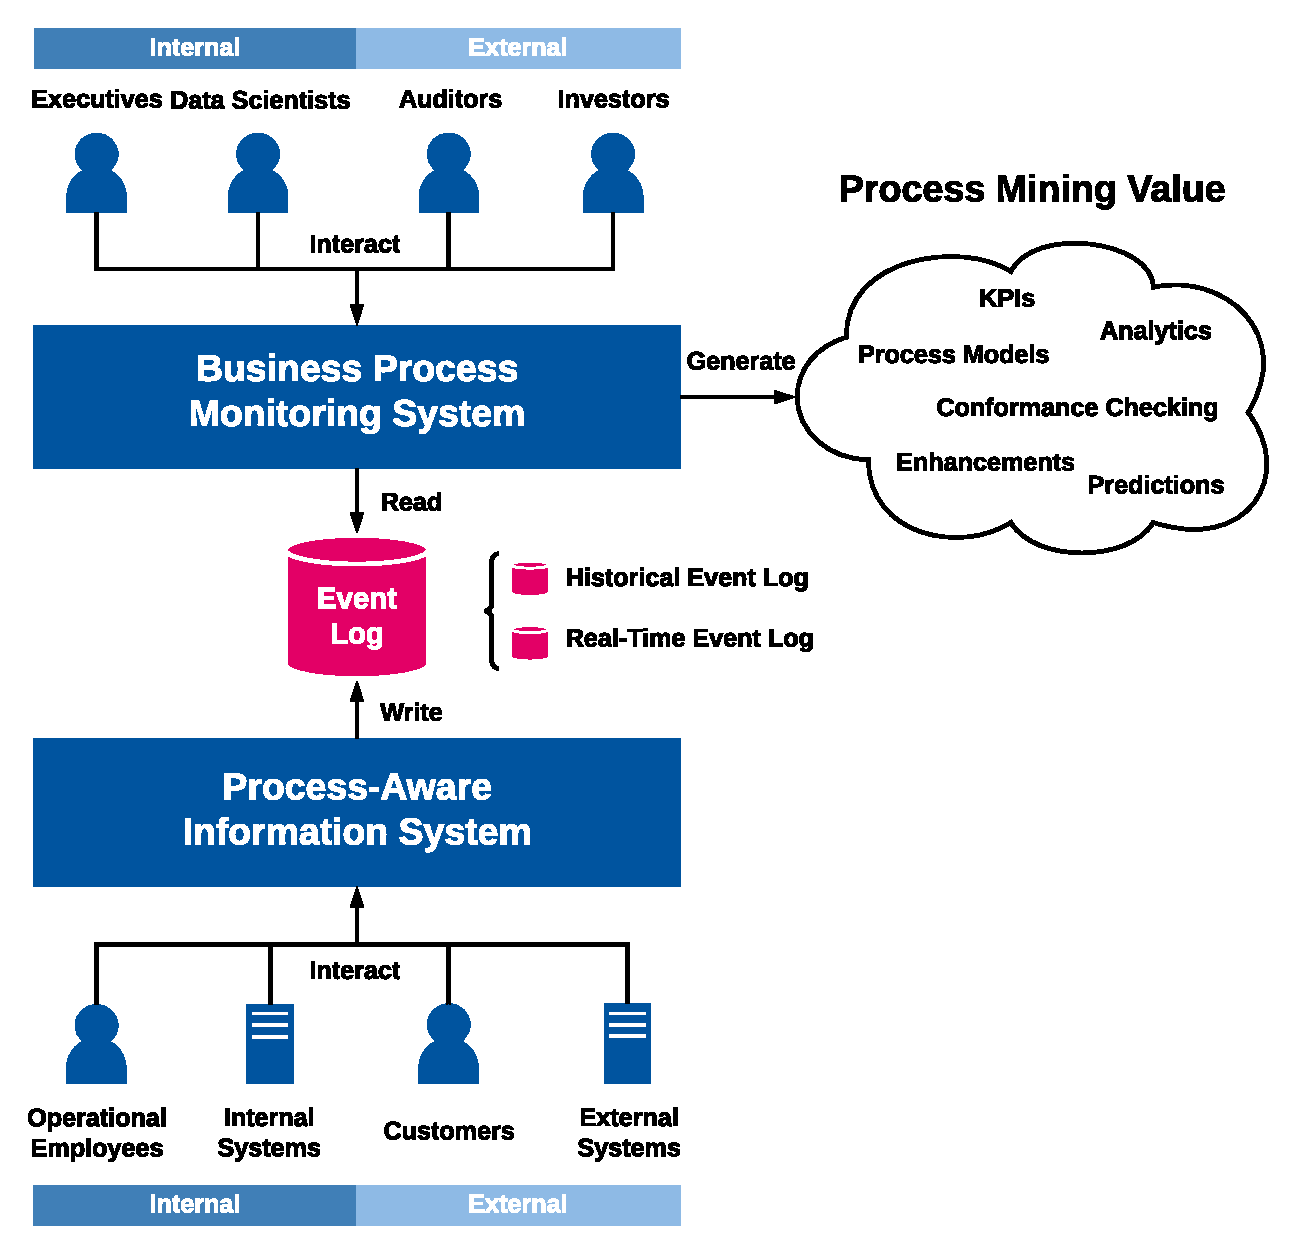
\includegraphics[width=\textwidth]{figures/process-monitoring}
	\caption{Business process monitoring allows to continuously apply process mining in an automated fashion in order to generate value for internal and external process stakeholders using the event data generated by an process-aware information system.}
	\label{fig:process-monitoring}
\end{figure}

Traditional process mining tends to be backward-looking \cite{DBLP:conf/scsc/Aalst18}, i.e. the focus relies on analyzing and understanding past executions of a process rather than providing value for running process instances in form of predictions or recommendations.
Businesses can develop a competitive advantage, if their process mining solution offers predictive capabilities, that allow to predict the future of a running process instance.
For example, if it is known beforehand, that a running process instance will probably exceed its deadline, measures can be initiated before damage occurs.
Therefore, including the forward-perspective is crucial for a competitive process mining software, especially in the context of business process monitoring.

\section{Problem Statement}

Although, many approaches for process prediction have been suggested in the literature (see Chapter \ref{chap:related_work}), current solutions are limited regarding the data they are able to consider and the targets they predict.
Many approaches derive the prediction purely from the control flow of process instance ignoring additional data attributes in the event log.
Especially, almost no approach is able to consider textual data for process prediction.
However, textual data can hold important information, that may be used to improve the prediction results.
In addition, most of the prediction methods focus on a single prediction dimension only, for example they just predict the remaining time until a process instance is finished.
But depending on the context also information about the next event or the future path of process instance can be of interest.
In some scenarios, processes instances have an outcome like success/failure or accepted/declined that can be predicted.

Precisely, given an event log with past executions of a process and a running (i.e. not completed) process instance, we would like to answer the following questions:

\begin{tabular}{ll}
	\textbf{Question} & \textbf{Prediction Target} \\
	What will happen next? & Next Activity\\
	When will it happen? & Next event time\\
	What is the most likely future path of the instance? & Future path\\
	When will the instance finish? & Remaining time\\
	What is the outcome of the instance? & Case outcome
\end{tabular}

\begin{figure}[htbp!]
	\centering
	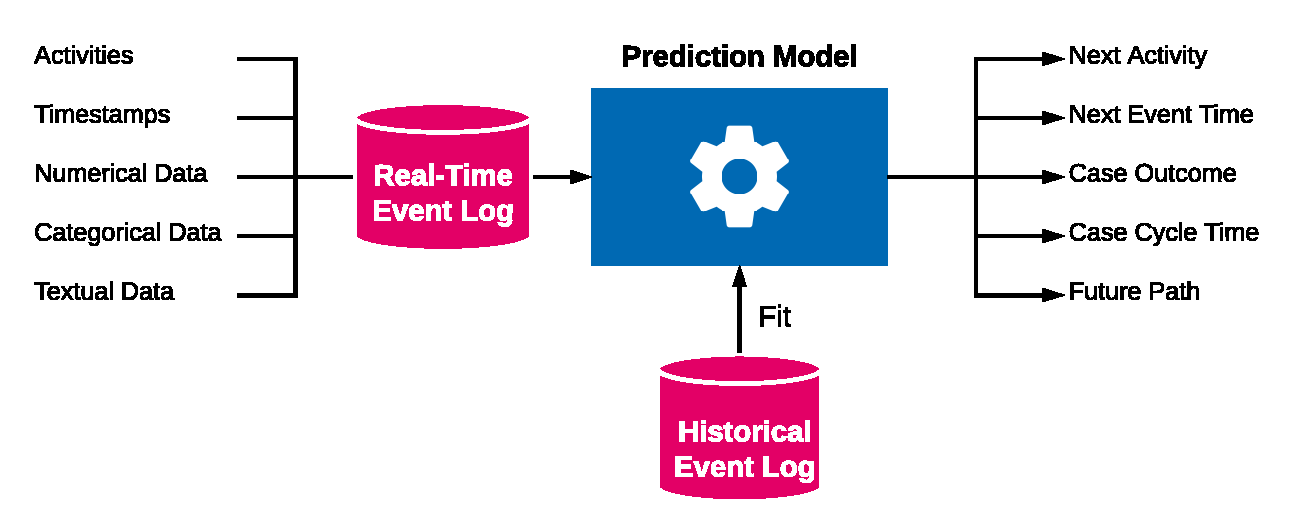
\includegraphics[width=\textwidth]{figures/problem-description}
	\caption[hello]{Predictive business process monitoring includes a prediction engine, that is able to predict the future of running cases using historical event data. Current approaches differs in terms of the considered input data, the underlying prediction model and prediction targets.}
	\label{fig:/problem-description}
\end{figure}

$\dots$

\section{Research Goals and Questions}

This thesis aims to improve current state-of-art approaches for process prediction in order to extend the capabilities of process monitoring software.
The main research goal is to design, implement and evaluate a predictive model for event data that is able to take advantage of additional textual data associated with each event.
Since most current approach are not able to handle textual data, we would like to know to what extend textual data can improve the quality of process prediction.
Furthermore, we want to evaluate different design choices and text models for text-aware process prediction and discuss potential trade-offs.
Lastly, we wan

These goals lead to the formulation of the following three research questions:

\begin{tabularx}{\textwidth}{lX}
	\textbf{RQ1} & To what extend can the utilization of textual data improve the performance of process prediction? \\
	\textbf{RQ2} & How does the choice of the text model and other parameters influence the prediction results?\\
	\textbf{RQ3} & What are the advantages and disadvantages of the approach compared to existing methods?
\end{tabularx}

\section{Contribution}



\section{Thesis Structure}

This thesis is structured in seven chapters.
In Chapter \ref{chap:prelim} the notations, definitions and concepts used in this contribution are introduced.
This includes an introduction to process mining, text mining, supervised learning and LSTM neural networks.
Chapter \ref{chap:related_work} summarizes relevant scientific contributions which focus on the problem of prediction in process mining and gives an overview of already available methods and their capabilities.
In Chapter \ref{chap:concept} the novel text-aware process prediction model as main conceptional contribution is presented.
Moreover, Chapter \ref{chap:impl} covers the implementation details of the model on a technical level.
In Chapter \ref{chap:eval} the performance of the new approach is evaluated and compared to current state-of-the-art prediction methods.
Finally, in Chapter \ref{chap:conclusion} the conclusion is given by wrapping up the key results as well as discussing the limitations of the approach.
Furthermore, an outlook towards future potential research questions on process prediction in the context of business process monitoring is given.

\chapter{Related Work} \label{chap:related_work}

The prediction of the future behavior of an process instance has been an important sub-field in the process mining research, that aims to enhance process monitoring capabilities.
Depending on the use case e.g. predicting time-related attributes, the future path or the the outcome of a case can be of interest. 
Most approaches presented in the literature either use machine learning based or process models based methods.

\Citeauthor{DBLP:conf/otm/DongenCA08} presented five different non-parametric regression predictors for forecasting the total cycle time of an unfinished case\cite{DBLP:conf/otm/DongenCA08}.
The estimates are based on activity occurrences, activity duration and attributes.

\Citeauthor{DBLP:journals/is/AalstSS11} proposed to build a transition system using a set, bag or sequence abstraction, which is annotated with time-related data in order to predict the remaining time of case \cite{DBLP:journals/is/AalstSS11}.
The core idea of this approach is to focus on the already completed cases, which are in some way most similar to new observed case.

\citeauthor{DBLP:journals/computing/PolatoSBL18} presented a set of approaches that use support vector regression for remaining time prediction\cite{DBLP:journals/computing/PolatoSBL18}.
In this work the authors implement different encoding for events including simple one-hot-encoding and a more advanced state based encoding using transition systems.
Furthermore, they enhance the approach in  \cite{DBLP:journals/is/AalstSS11} by taking additional data attributes into account.

Most recently, several authors have applied recurrent neural networks in form of LSTM networks for process prediction. \citeauthor{ DBLP:conf/bpm/EvermannRF16} encode events using an embedding matrix as it is known for word embeddings. The embedded events are then used as input for an LSTM network that predicts the next activity\cite{DBLP:conf/bpm/EvermannRF16}.

\citeauthor{DBLP:conf/caise/TaxVRD17}] use an one-hot-encoding of the activity and the timestamp of an event to predict the activity and timestamp of the next event. This is done by using a two-layered LSTM network\cite{DBLP:conf/caise/TaxVRD17}.

More recent work by \citeauthor{DBLP:conf/ssci/NavarinVPS17} adopts this idea and extends the encoding to additional data attributes associated with each event\cite{DBLP:conf/ssci/NavarinVPS17}.

\citeauthor{DBLP:conf/bpm/TeinemaaDMF16} applied text vectorization techniques like bag of n-grams (BoNG), Latent Dirichlet Allocation (LDA) and Paragraph Vectors (PV) to textual data of processes in order to predict a binary label describing the process outcome\cite{DBLP:conf/bpm/TeinemaaDMF16}. In this approach random forest and logistic regression classifiers for each prefix length of a trace are trained.

\chapter{Preliminaries} \label{chap:prelim}
In this chapter the basic concepts of process mining, text mining, supervised learning and long short-term memory networks are presented. Furthermore, necessary formal definitions and notations are introduced.


\section{Processes and Process Mining}

A \textit{business process} is a collection of activities that are performed in a specific order to archive a goal \cite{DBLP:conf/bpm/AalstAM11}.
A single execution of a process is a \textit{case} or \textit{process instance}, which is identified by a case ID.
Each performed activity belongs to specific case and is completed at a certain time.
A case can be for example a patient in a hospital, a customer journey or an online order. The time on which an activity for a certain case is performed is specified by a timestamp.
The trinity of case, activity and timestamp is called \textit{event}.
An event can have more attributes, for example resource, costs or transactional information.

\begin{table}[htbp!]
	\small
	\setlength\tabcolsep{3pt}
	\begin{tabularx}{\textwidth}{lllllp{4.7cm}l}
		\toprule
		\textbf{ID} & \textbf{Activity}          & \textbf{Timestamp} & \textbf{Resource} & \textbf{Cost} & \textbf{Comment}  \\
		\midrule
		0                & Register patient           & 01.02.2020:14.12   & SYSTEM            & 0             & -     \\
		& Consultation               & 01.02.2020:14.34   & J. Brown, MD    & 24.32         & The patient reports persistent nausea.   \\
		& Blood test                 & 01.02.2020:15.12   & K. Smith         & 14.23         & Tests: Complete blood count    \\
		& Evaluate test  & 01.02.2020:16.35   & J. Brown, MD    & 38.67         &No abnormalities in the complete blood count.   \\
		& Release patient            & 01.02.2020:17.24   & SYSTEM            & 0             & -  \\
		&                            &                    &                   &               &     \\
		\midrule
		1                & Register patient           & 02.02.2020:08.20   & SYSTEM            & 0             & -  \\
		& Consultation               & 02.02.2020:14.12   & J. Simpson, MD  & 24.32         & Noticeable tachycardia. No chronic pre-existing conditions are known.    \\
		& MRI & 02.02.2020:14.12   & Sara Taylor, MD   & 352.87        & -    \\
		& Release patient            & 02.02.2020:14.12   & SYSTEM            & 0             & -   \\
		&                            &                    &                   &               &     \\
		\midrule
		2                & Register patient           & 02.02.2020:09.08   & SYSTEM            & 0             & -    \\
		& Consultation               & 02.02.2020:09.14   & J. Simpson, MD  & 24.32         & The patient has severe leg injuries due to a motorcycle accident.  \\
		& Hospitalization       & 02.02.2020:09.20   & M. Johnson      & 130.37        & -     \\
		...              & ...                        & ...                & ...               & ...           & ...     \\ \bottomrule
	\end{tabularx}
	\caption[Artificial event log of patient treatments in a hospital]{Artificial event log of patient treatments in a hospital. Each line corresponds to one event. The events are grouped by their case IDs, that each represent a single patient.}
	\label{tab:event-log}
\end{table}

If the execution of a business process is logged by an information system, the resulting event data is called \textit{event log}.
Depending on the format of the event log, it can also contain additional data on case level.
Typical formats for event logs, are comma-separated values (CSV) and eXtensible Event Stream (XES) \cite{DBLP:conf/caise/VerbeekBDA10a}, which can be extracted from databases.
A table-based representation of an artificial event log about patient treatment in a hospital can be seen in Table \ref{tab:event-log}.
Besides the case ID, activity and timestamp, the event log also contains information about the identity executing the activity, the costs of the activity and a text comment in form of a categorical, numerical and textual attribute.

Process mining is the discipline that covers all approaches aiming to generate value out of event data.
As an umbrella term, process mining includes or utilizes concepts of business process management, data mining, business process intelligence, big data, workflow management, business process monitoring \cite{DBLP:books/sp/Aalst16} as well as machine learning \cite{DBLP:conf/bpm/VeitGMHT17}.

Traditionally, process mining is divided into a set of subdisciplines mainly process discovery, conformance checking, process enhancement and process analytics \cite{DBLP:conf/caise/EckLLA15}.
Process discovery aims to generate process models out of event data in order to understand a process and enable further analysis.
Conformance checking is about comparing the intended and observed behavior of a process and identifying deviations.
On top of these diagnostic approaches, process enhancement deals with the improvement of processes regarding compliance, performance or complexity.

Finally, process analytics focuses on metric and performance evaluation of processes. Similar to conformance checking, this term is closely related to business process monitoring, a rising subfield enabling the analysis of running business processes in real-time.
Driven by the fast and ongoing development of quantitative prediction methods in data science and machine learning, also prediction-based methods have been applied to event data.
These methods add the forward perspective to business process monitoring and deal with forecasting the future of a running process instance, which is also the main focus of this work.


\section{Basic Notations and Sequences}

The set $\mathbb{N}$ denotes the set of all natural numbers $\{1, 2, 3, \dots\}$ and $\mathbb{N}_0 = \mathbb{N} \cup \{0\}$ denotes the set of natural numbers including 0.
The set of natural numbers up to $n$ is noted as $[n] = \{1, 2, \dots, n\} \subset \mathbb{N}$ with [0] = $\emptyset$.

\begin{definition}[Sequence]
		A \textit{sequence} of length $n \in \mathbb{N}_0$ over a set $A$ is an ordered collection of elements defined by a function $\sigma \colon [n]\to A$, which assigns each index an element of $A$.
		A sequence  of length $n$ is represented explicitly as $\sigma = \langle a_1, a_2, \dots, a_n\rangle $ with $a_i \in A$ for $1 \leq i \leq n$. In addition, $\langle \rangle$ is the empty sequence of length $0$.
\end{definition}

Given a set $A$, $A^n$ describes the set of all sequences $\langle a_1, a_2, \dots, a_n\rangle$ over $A$ of length $n$.
The set $A^0$ is defined as $\{\langle \rangle\}$, the set that only contains the empty sequence.
The set of all possible sequences over $A$ is given with $A^* = \bigcup\limits_{i\in \mathbb{N}_0} A^i$.

Given sequences $\sigma_1$ and $\sigma_2$, the concatenation of both sequences is denoted by $\sigma_1 \cdot \sigma_2$.
Moreover, the $i$-th element of a sequence $\sigma = \langle a_1, a_2, \dots, a_n\rangle$ is accessed using $\sigma(i)= a_i$ for $1 \leq i \leq n$.
The length of a sequence is denoted by $|\sigma|$.
For a sequence $\sigma=\langle a_1, a_2, \dots, a_n\rangle$, the function
$hd^k(\sigma)= \langle a_1, a_2, \dots, a_k\rangle$ gives the prefix of length $k$ of $\sigma$ and $tl^k(\sigma)= \langle a_{k+1}, a_{k+2}, \dots, a_n\rangle$ the suffix of length $n-k$ for $0 \leq k \leq n$.
%Note that $\sigma = hd^k(\sigma) \cdot tl^{n-k+1}(\sigma)$ for corresponding $k$.
%If an element $a_i \in A$ appears in a sequence $\sigma$, we also write $a_i \in \sigma$.

A function $f \colon A \to B$ can be lifted element-wise to sequences over $A$, precisely:
\begin{equation*}
f(\sigma) =
\begin{cases}
\langle \rangle & \text{if $\sigma = \langle \rangle$} \\
\langle f(a_1), f(a_2), \dots, f(a_n)\rangle & \text{else} 
\end{cases}
\end{equation*}

\section{Events, Traces, Event Logs}

\begin{definition}[Event]
An  \textit{event} is defined by tuple $e = (a,c,t,d_1,\dots, d_m) \in \mathcal{C} \times \mathcal{A}  \times \mathcal{T} \times \mathcal{D}_1 \times \dots \times \mathcal{D}_m =  \mathcal{E}$ where  $c \in \mathcal{C} $ is the case ID, $a \in \mathcal{A}$ is the executed activity and $t \in \mathcal{T}$ is the timestamp of the event.
Furthermore, each event contains a fixed number $m \in \mathbb{N}_0$ of additional attributes $d_1 \dots d_m$ in their corresponding domains $\mathcal{D}_1, \dots , \mathcal{D}_m$.
In case that no additional attribute data is given ($m = 0$) the event space $\mathcal{E}$ (set of all possible events) is reduced to $\mathcal{C} \times \mathcal{A}  \times \mathcal{T}$.
\end{definition}

Each attribute $d \in \mathcal{D}$ of an event (including activity, timestamp and case ID) can be accessed by a projection function $\pi_D \colon \mathcal{E} \to \mathcal{D}$.
For example, the activity $a$ of an event $e$ is retrieved by $\pi_\mathcal{A}(e) = a$.

Throughout this thesis,  $\mathcal{C} = \mathbb{N}_0$, $|\mathcal{A}| < \infty$ and $ \mathcal{T} = \mathbb{R}$ is assumed, where $t \in \mathcal{T}$ is given in Unix time, precisely the number of seconds since 00:00:00 UTC on 1 January 1970 minus the applied leap seconds.
Each additional attribute is assumed to be numerical, categorical or textual, i.e. $\mathcal{D}_i = \mathbb{R}$, $|\mathcal{D}_i| < \infty$ or $\mathcal{D}_i = V^\ast$  for $1 \leq i \leq m$ and some fixed vocabulary $V$.

\begin{definition}[Trace]
	A \textit{trace} is a finite and non-empty sequence of events $\sigma = \langle e_1, e_2, \dots\rangle \in  \mathcal{E}^\ast$ with increasing timestamps, i.e. $\pi_\mathcal{T} (e_i) < \pi_\mathcal{T} (e_j) $ for $1 \leq i < j \leq |\sigma|$.
\end{definition}


By lifting the projection functions to sequences a trace can be transformed into a sequence of attributes by applying the projection function to the trace.
For example, $\pi_\mathcal{A}(\sigma)$ gives the sequence of the activities of the events in $\sigma$.

\begin{definition}[Event log]
	An \textit{event log} or \textit{trace log} $\eventlog = \{ \sigma_1, \sigma _2, \dots, \sigma_k \}$ is a set of traces, where each event of a trace is unique in the log and all events of a trace share a case IDs, which is unique per trace.
\end{definition}

\section{Text Mining}

\textit{Text mining} describes all techniques to generate value out of unstructured or semi-structured textual data.
It combines concepts of natural language processing, machine learning and data mining \cite{DBLP:journals/coling/Mihalcea08}.
The base object in text mining is a \textit{document} containing textual data.
The textual data can be completed unstructured, i.e. it does not conform to a pre-defined data model, or semi-structured, like in an e-mail, where text information is assigned to sender, subject, message etc.
In our setting, a document $d \in V^*$ (i.e. textual data) is always a sequence of words from a fixed vocabulary $V$.
A collection of documents is called \textit{text corpus}, which forms the basis for many text mining techniques.

In order to derive a mathematical representation of the text data that can be interpreted by a computer, a text model has to be build using the text corpus.
Popular text models are Bag-of-words, Bag-of-n-gram, Paragraph vector (a.k.a. Doc2Vec) \cite{DBLP:conf/icml/LeM14} and Latent Dirichlet Allocation \cite{DBLP:journals/jmlr/BleiNJ03}.
Most models do not work with the raw text data, but require a text normalization step, where the text is cleaned from linguistic variation as well as meaningless words and symbols \cite{DBLP:books/lib/JurafskyM09}.

\section{Supervised Learning}

In \textit{supervised learning} an unknown function is learned (i.e. approximated) from a set of example input-output pairs \cite{DBLP:books/daglib/0023820}.
In contrast, \textit{unsupervised learning} does not require examples pattern and is about finding pattern in the data. 
An input instance is usually described by a set of \textit{feature variables} $X$ and the output is defined by a \textit{target variable} $y$.
If the target variable $y$ is continuous, we refer to this as a regression problem, if however it is discrete variable with a finite range of values, the learning problem is called classification problem.
Given a \textit{training set} of input-output pairs $\{(X_1, y_1), (X_2, y_2), \dots, (X_m,y_m)\}$, that were generated from an unknown function $y = f(X)$, the goal is to approximate a hypothesis function $h(X)$, which is close to f(X), i.e. $h(X) \approx f(X)$.

The challenge in supervised learning is to generalize from the training set of input-output pairs in such a way, that the learned hypothesis function $h(x)$ can also successfully predict the target variable for unseen problem instances.
In order to evaluate a hypothesis, the function is tested on a separate \textit{test set} of input-output pairs, which has not been used for the construction of $h(X)$.

A hypothesis is assumed to generalize well, if its prediction performance is high on the training set as well as on test set.
However, if the prediction performance is high on the training set, but not reliable on unseen data, the hypothesis might \textit{overfit} the training data.
In this case, the model complexity, i.e. the number of parameters is higher than justified by the true function. 
In contrast, if the model is too simple to fit any data from training set, the hypothesis is \textit{underfitting}.

In many real-world applications, the true function $f(X)$ is stochastic, i.e. we need to estimate a conditional probability function $P(Y | X)$ (classification problem) or a conditional expectation $E(Y | X)$ (regression problem) for prediction.
Therefore, the prediction accuracy is always limited by the randomness of the true distribution.
Typical supervised learning algorithms are linear regression, support vector machines, decision trees or neural networks including long short-term memory networks.
\section{Long Short-Term Memory Networks}

Long short-term memory (LSMT) is an advanced recurrent neural network architecture for sequential data originally presented by \citeauthor{DBLP:journals/neco/HochreiterS97} in \citeyear{DBLP:journals/neco/HochreiterS97}  \cite{DBLP:journals/neco/HochreiterS97}.
This approach addresses the well-known vanishing and exploding gradient problem \cite{DBLP:conf/icml/PascanuMB13}  of traditional recurrent neural networks by introducing more complex LSTM cells as hidden units.
The proposed architecture has been improved several times \cite{DBLP:journals/neco/GersSC00} \cite {DBLP:journals/tnn/GreffSKSS17} and considered as one of the most successful recurrent neural network models.
Although LSTM networks have been available for a long time, the breakthrough of this technology is dated around 2016 after many success stories of LSTM in combination with large data sets and GPU hardware have been reported for sequence to sequence tasks like text translation \cite{DBLP:journals/corr/WuSCLNMKCGMKSJL16}.

Gated recurrent units (GRU) \cite{DBLP:conf/emnlp/ChoMGBBSB14} are the competing gating mechanism by \citeauthor{DBLP:conf/emnlp/ChoMGBBSB14} that have fewer parameters and perform similar to LSTM.
However, more recent studies show, that LSTM outperforms GRU consistently in neural machine translation tasks \cite{DBLP:journals/corr/BritzGLL17}.

A simple feedforward neural networks consists of an input layer, arbitrarily many hidden layers and an output layer, where each layer consists of neurons that compute and output the weighted sum of the cells of the previous layer that has been passed to an non-linear activation function \cite{DBLP:journals/nn/Schmidhuber15}.
These networks can learn and compute complex functions in supervised learning settings, where input and output pattern are provided.
The network computes a loss function for each training pattern and adjusts its weights with gradient descents using a back-propagation algorithm in order to minimize the loss function \cite{rumelhart1986learning}.

Recurrent neural networks extend traditional feed forward networks with backfeeding connections between hidden layers.
This enables the network to keep a state across inputs and allows the neural network to process arbitrarily long sequences of input data while learning temporal dependencies.

In LTSM networks the layers are replaced by more complex LSTM modules, where each module contains four different sublayers.
The module uses as input the state $\vec{c}_{t-1}$ and the hidden output $\vec{h}_{t-1}$ of the module in the previous time step as well as the output of the previous layer $\vec{x}_t$ to compute a new cell state $\vec{c}_{t}$ and a (hidden) output $\vec{h}_{t}$.

\begin{figure}[htbp!]
	\centering
	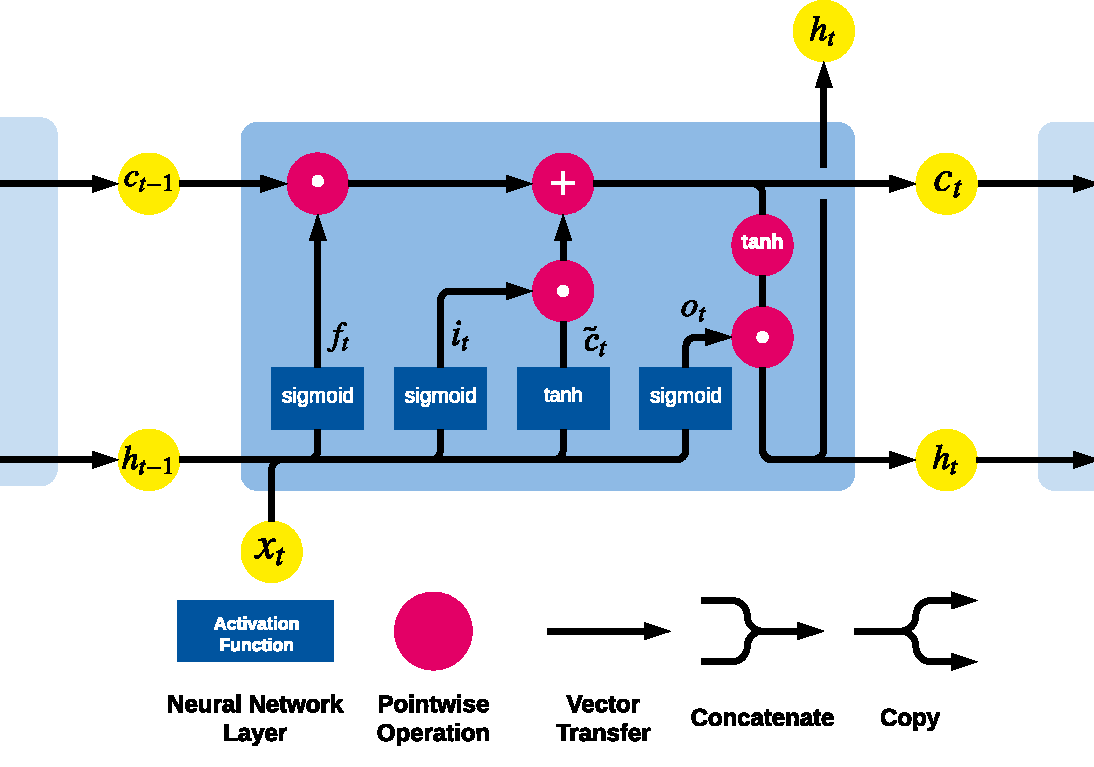
\includegraphics[width=0.9\textwidth]{figures/lstm-module}
	\caption[Structure of an LSTM module]{LSTM module with four sublayers that manipulate the cell state and compute the module's output. Graphic adapted from \cite{lstm-blog}.}
	\label{fig:lstm-module}
\end{figure}


The input vector $\vec{x}_t$ is concatenated with the previous hidden output $\vec{h}_{t-1}$ and fed to four neural network layers, which are designed to decide what part of the cell state will remain (forget gate $\vec{f}_t$), how it is updated (update gate $\vec{i}_t$ and $\vec{\bar{c}}_t$) and what the output of the layer will be (output gate $\vec{o}_t$ leading to $\vec{h}_t$).
The sublayer apply $\text{sigmoid}(x) = \frac{1}{1+\exp({-x})}$ or $\tanh(x) = \frac{\exp({x}) - \exp({-x})}{\exp({x}) + \exp({-x})}$ activation functions elementwise, leading to the following equations:

\begin{equation*}
	\vec{f}_t = \text{sigmoid}(\vec{W}_f \cdot (\vec{h}_{t-1}, \vec{x}_t) + \vec{b}_f)
\end{equation*}

\begin{equation*}
	\vec{i}_t =  \text{sigmoid} (\vec{W}_i \cdot (\vec{h}_{t-1}, \vec{x}_t) + \vec{b}_i)
\end{equation*}

\begin{equation*}
	\vec{\bar{c}}_t = \tanh (\vec{W}_c \cdot (\vec{h}_{t-1}, \vec{x}_t) + \vec{b}_c)
\end{equation*}

\begin{equation*}
	\vec{o}_t =  \text{sigmoid} (\vec{W}_o \cdot (\vec{h}_{t-1}, \vec{x}_t) + \vec{b}_o)
\end{equation*}

$\vec{W}_f$, $\vec{W}_i$, $\vec{W}_c$ and $\vec{W}_o$ are the sublayer's learned weights and $\vec{b}_f$, $\vec{b}_i$, $\vec{b}_c$ and $\vec{b}_o$ are the corresponding biases.

The new cell state $\vec{c}_t$ is then a combination of the old cell state $\vec{c}_{t-1}$ and the result of the update gate $\vec{\bar{c}}_t$, where the layer computations $\vec{f}_t$ and $\vec{i}_t$ determine the proportions by a pointwise multiplication ($\odot$) with the cell states.

\begin{equation*}
	\vec{c}_t = f_t \odot \vec{c}_{t-1} + \vec{i}_t \odot \vec{\bar{c}}_t
\end{equation*}

The result of the output gate $\vec{o}_t$ is pointwise multiplied with the tanh-activated new cell state to calculate the hidden output $\vec{h}_t$ of the module.

\begin{equation*}
	\vec{h}_t = \vec{o}_t \odot \tanh(\vec{c}_t )
\end{equation*}

LSTM networks are able to backpropagate a more stable error with this gating mechanism, such that these networks are much more capable of learning complex functions for sequences compared to standard recurrent neural networks.

\chapter{Concept} \label{chap:concecpt}
Text-aware process prediction aims to utilize unstructured text information in event data to improve case predictions.
While many prediction methods have been applied to event data, almost none of them are able to handle textual data.
An exception is the approach presented in \cite{DBLP:conf/bpm/TeinemaaDMF16}, where traces are encoded as fixed vectors and a classifier is learned for each prefix length.

In this chapter a novel approach for process prediction is presented that is able to handle numerical, categorical and textual data, captures temporal dependencies and concept drifts using an event-wise encoding and a sequential prediction model (LSTM).

\section{Overview}





\section{Event Encoding}

\subsection{Encoding of Activities and other Categorical Attributes}

\subsection{Encoding of Time and other numerical Attributes}

For timestamp prediction of the next and final event of running process instance a set of time-based features is computed from the timestamp data in the event log.
Given an event log $\eventlog$ an event $e_i$ from a trace $\sigma = \langle e_1, \dots, e_n \rangle$ the following time features are computed for the encoding of $e_i$: 

\begin{center}
\begin{tabularx}{\textwidth}{l l}
	\centering
	 \textbf{Feature} & \textbf{Description} \\
	$t_1 = \pi_\mathcal{T}(e_i) - \pi_\mathcal{T}(e_{i-1})$ & Seconds since previous event \\
	$t_2 = \pi_\mathcal{T}(e_i) - \pi_\mathcal{T}(e_1)$ & Seconds since case start \\
	$t_3 = \pi_\mathcal{T}(e_i) - \min\{\pi_\mathcal{T}(e_{j}), \forall e_j \in \sigma_k, \forall  \sigma_k \in \eventlog\}$ & Seconds since first recorded event \\
	$t_4$ & Seconds since midnight \\
	$t_5$ & Seconds since last Monday \\
	$t_6$ & Seconds since last January 1 00:00
\end{tabularx}
\end{center}

Using the time features a set of time-dependent trends can be captured and utilized for prediction.
The features $t_1$ and $t_2$ give information about the time between events and the time of the event in the case.
Using $t_3$ the absolute time position of an event in the data can be determined.
This is important to detect concept drift in the process.
The features $t_4, t_5$ and $t_6$ are used to capture daily, weekly or seasonal trends.
For example, some activities might only be executed during office hours, before the weekend, during summer.

Each feature $t_1, \dots t_6$ as well as all additional numerical attributes $d_i$ are scaled to the interval $ [0, 1]$ to improve learning efficiency using min-max normalizing.
The scaling for a numerical feature $x$ is realized with the transformation

$$\hat{x} = \dfrac{x-\min(x)}{\max(x) - \min(x)} \in [0, 1],$$

where $\min(x)$ is the lowest and $\max(x)$ is the highest value $x$ can take.
If the limits are not bounded conceptually, the lowest or highest value of $x$ in the event log is used for scaling.

\subsection{Text Encoding}

In order to prepare the textual data of the event log for a prediction model, the texts have to be encoded in a "useful" numerical vector representation.
Useful in that context means, that texts with similar semantic meanings should also have similar representations.
Extracting the meaning of textual information remains a challenge even for humans, because textual data is unstructured, language dependent and domain specific.
In addition, grammatical variations and the importance of context in language makes text mining even more difficult.

The text vectorization is realized in a 2-step procedure.
First, all text data associated with the events in the corresponding textual attribute is collected in a so called \textit{text corpus}.
Each document in the text corpus is then preprocessed in order to filter out linguistic noise or useless information.
Finally, the text corpus is used to build up a vocabulary and a text vectorization technique is applied to encode the text attribute to a fixed of vector.

\subsubsection{Text Preprocessing}

In the preprocessing step each document is transformed by a processing pipeline which consists of the following four steps:

\begin{enumerate} 
	\item Letters are converted to lowercase
	\item Document is tokenized by word
	\item Each word is lemmatized
	\item Stop words are filtered out
\end{enumerate}

In the tokenenization step a document is split up in a list of words.
Each word is then lemmatized, i.e. it is converted to its canonical form.
The idea is to unify words that have a very similar meaning and filter out grammatical variations.
For example, the words  "go", "going", "goes", "gone" and "went" are all transformed to the basic form "go".
Ultimately, all stop words are filtered out of each document.
Stop words are words with low information value like "the", "a", "of" or "here".

Stop word lists are language dependent and can be more or less aggressive at filtering.
Usually they contains articles, auxiliary verbs, prepositions and generic verbs like "be" and "have".
In addition, punctuation marks or numerical information are excluded.

\begin{table}[]
	\begin{tabularx}{\textwidth}{l l p{9.8cm}}
		\toprule
		\textbf{Step} & \textbf{Transformation} & \textbf{Document}                                                       \\ \midrule
		0             & Original       & "The patient has been diagnosed with high blood pressure." \\
		1             & Lowercase               & "the patient has been diagnosed with high blood pressure." \\
		2 & Tokenization  & {[}"the", "patient", "has", "been", "diagnosed", "with", "high", "blood", "pressure", "."{]} \\
		3 & Lemmatization & {[}"the", "patient", "have", "be", "diagnose", "with", "high", "blood", "pressure", "."{]}   \\
		4             & Stop word filtering     & {[}"patient", "diagnose", "high", "blood", "pressure"{]} \\ \bottomrule
	\end{tabularx}
	\caption{Preprocessing transformation of an example document}
	\label{tab:text-preprocessing}
\end{table}








\subsubsection{Bag-of-N-Gram}
\subsubsection{Paragraph Vector}

\section{Network}

\chapter{Implementation} \label{chap:impl}
This chapter covers the implementation of the text-aware process prediction model presented in the previous chapter.
In Section \ref{sec:technology} the underlying technology is depicted, whereas in Section \ref{sec:model-implementation} the architecture of the implementation is defined.

\section{Technology}\label{sec:technology}

The implementation of the text-aware process prediction model is purely based on Python 3.6 \cite{python}.
The set of Python packages that are utilized for the implementation are summarized in Table \ref{tab:packages}.
All packages follow the open-source development model and are mostly community-driven.

\begin{table}[!htbp]
	\begin{tabularx}{\textwidth}{l p{4.5cm} p{6.6cm} }
		\toprule
		\textbf{Package} & \textbf{Developer(s)} & \textbf{Purpose}  \\
		\midrule
		PM4Py \cite{DBLP:journals/corr/abs-1905-06169}   &  Fraunhofer Institute for Applied Information Technology &  Event log parsing and handling\\
		TensorFlow \cite{DBLP:journals/corr/AbadiABBCCCDDDG16} &  Google Brain Team et al.& Construction and training of LSTM model \\
		NTLK \cite{DBLP:books/daglib/0022921} & Bird et al. & Text preprocessing\\
		Scikit-learn \cite{DBLP:journals/jmlr/PedregosaVGMTGBPWDVPCBPD11} & Cournapeau et al.& Bag of Words and Bag of N-Gram tf-idf encoding \\
		Gensim \cite{rehurek_lrec} & Řehůřek et al. & Latent Dirichlet Allocation and Paragraph Vector encoding \\
		 \bottomrule
	\end{tabularx}
	\caption[List of Python packages used for implementation]{List of Python packages used for implementation.}
	\label{tab:packages}
\end{table}

PM4Py \cite{DBLP:journals/corr/abs-1905-06169} is a Python package developed by the Fraunhofer Institute for Applied Information Technology, which offers a wide range of process mining algorithms and event log operations for the Python environment.
It is used for event log parsing and its internal event log representation.

TensorFlow \cite{DBLP:journals/corr/AbadiABBCCCDDDG16} is a dataflow oriented framework originally developed by Google, which includes a diverse set of neural network models and serves with its LSTM implementation using the Keras API \cite{chollet2015keras}.

Furthermore, the packages NTLK \cite{DBLP:books/daglib/0022921}, Scikit-learn \cite{DBLP:journals/jmlr/PedregosaVGMTGBPWDVPCBPD11} and Gensim \cite{rehurek_lrec} are applied for the preprocessing and encoding of textual data.
NTLK is used to realize the tokenization and word lemmatization, whereas the implementation of the text models is supported by the Scikit-learn (Bag of Words, Bag of N-Gram) and Gensim (LDA, Paragraph Vector) packages.


\section{Model Implementation}\label{sec:model-implementation}

The interface of the text-aware process prediction model (tapp) is realized through a class \texttt{TappModel}, which implements the functions \texttt{fit()},  \texttt{predict()} and  \texttt{evaluate()}, that can be used to fit the model to an event log with historical data, compute prediction for an event log with uncompleted traces and evaluate the performance of the prediction model.
The \texttt{TappModel} manages the underlying LSTM model and can be configured with the number of shared and specialized layers as well as the dimension of the hidden neurons per LSTM layer.

\begin{figure}[htbp!]
	\centering
	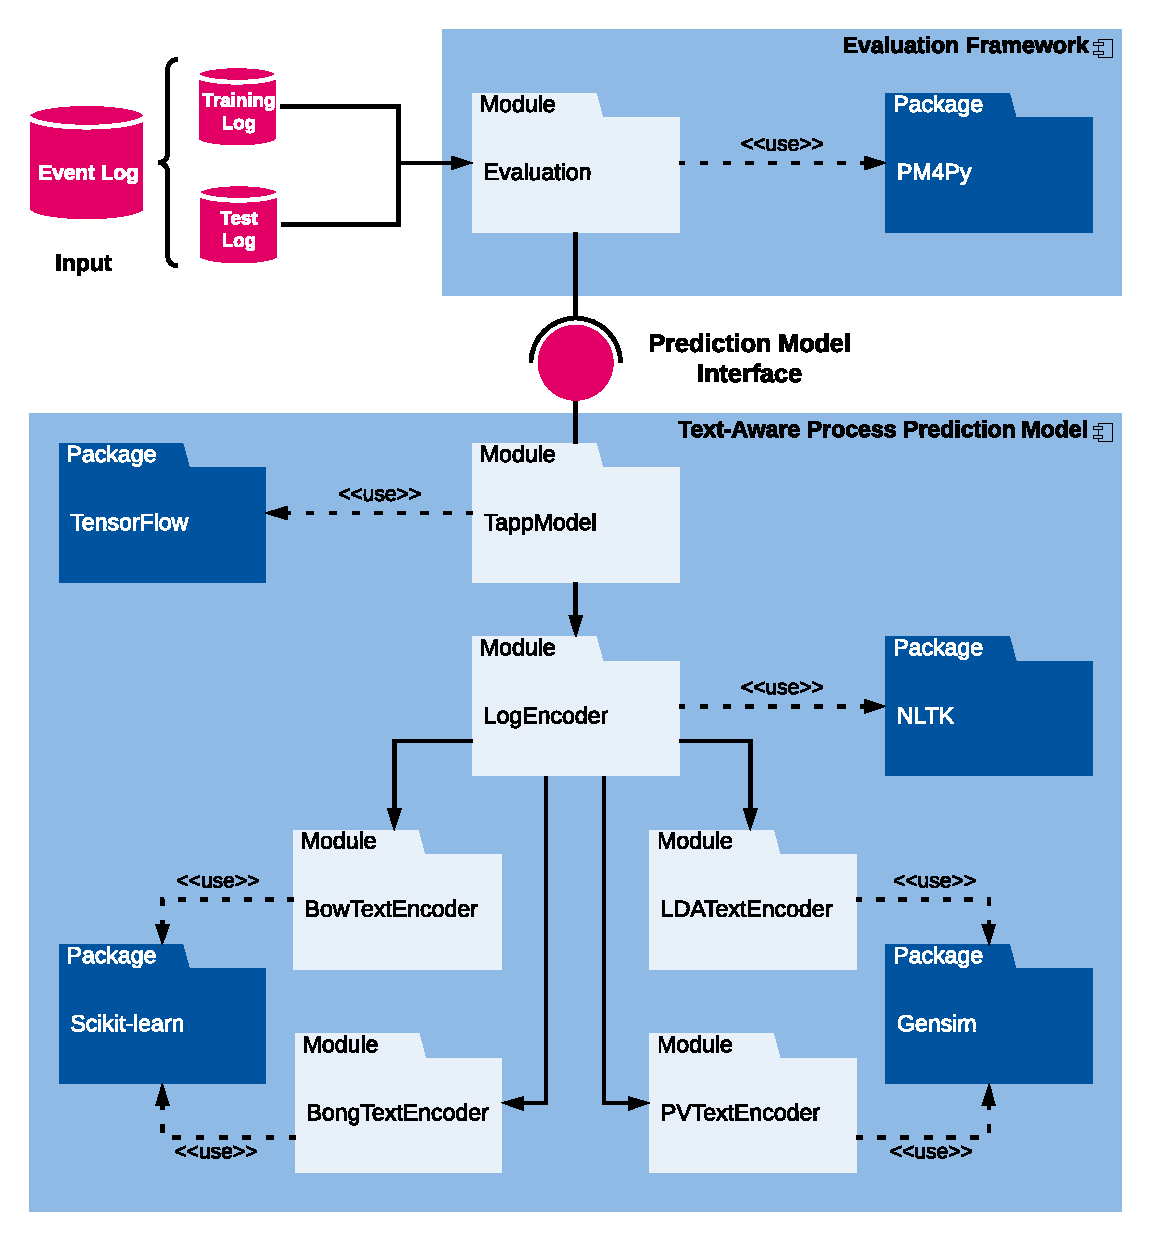
\includegraphics[width=\textwidth]{figures/implementation}
	\caption[Component diagram of the implementation]{Component diagram of the implementation.}
	\label{fig:/implementation}
\end{figure}

The encoding of traces as described in Section \ref{sec:event}, \ref{sec:time} and \ref{sec:text} is computed in the \texttt{LogEncoder} module, which is controlled by the \texttt{TappModel}.
The \texttt{LogEncoder} is also fitted to the historical log and can transform (prefix) traces to the encoded matrix format via functions \texttt{fit()} and \texttt{transform()}.
It is configured with one out of the four text encoding models described in Section \ref{sec:text} (\texttt{BowTextEncoder},  \texttt{BongTextEncoder}, \texttt{LDATextEncoder} and  \texttt{PVTextEncoder}), that realizes the vectorization of textual data.
Just like the \texttt{LogEncoder}, the text encoding models offers the functions \texttt{fit()} and \texttt{transform()} adapt to the historical data and compute the text encoding.

During the fitting phase of the  \texttt{LogEncoder}, all possible values for categorical attribute are indexed and the parameters for the normalization of numerical attributes are computed.
With regard to the text encoding model, the indexed vocabulary of all words (after preprocessing) in the historical event log is built during fitting.
In case of the Paragraph Vector model, the encoding network is trained with the training corpus.

The text-aware process prediction model can be used in any business process monitoring software to provide the prediction capabilities using the methods of the \texttt{TappModel}.
In order to evaluate the performance of the model, an experiment using the \texttt{Evaluation} module is performed, which is described in-depth in Chapter \ref{chap:eval}.
The module reads an event log using PM4Py, divides it into a training and test log and measures the prediction performance of differently configured instances of the text-aware process prediction model.
An overview of the different components of the implementation is shown in Figure \ref{fig:/implementation}.

\chapter{Evaluation} \label{chap:eval}
In this chapter, the performance of the text-aware process prediction model is evaluated based on simulated and real-world event data.
First, the data sets and evaluation method are described. Then, the performance of differently parameterized models on the data sets is evaluated and analyzed in-depth.


\section{Data Sets}

The prediction model is evaluated on one simulated and two real-world event logs, which are described in the following.
An overview of the key properties of the logs is summarized in Table \ref{tab:logs}.

\textbf{Job Application} (Simulated) This event log describes a simple job application process. 
First, the applicant starts an application in the company's system.
Then, he or she uploads a curriculum vitae (CV) and optionally a cover letter in an random order.
When the documents have been received, the applicant is either directly rejected by the company or invited to an interview.
In case of an invitation the applicant responds in an email, if he or she would like to accept or reject the invitation.
After the interview a decision is made and sent to the applicant that states, if the applicant gets a job offer or is rejected.
in case of a job offer, the applicant answers in an email if he or she would like to accept the job offer.
Furthermore, noise is added by introducing a 1\% probability after each event that the process stops immediately.

The timestamp of each event is determined by sampling from a normal distribution, which mean and variance is unique per activity.
The CV, cover letter and all emails are available as a text attribute in the event log.
The text information is generated by sampling 10 times from sets of full and partial sentences depending on the control flow
For example, if an applicant gets a job offer, the generated email contains text fragments from typical job offer emails.
If on the other hand the applicant is rejected, the email is generated with sentences from typical rejection emails.
With this text generation mechanism, all texts in the event log are unique, but the words and sentences in the texts correlate with the path of the corresponding case.

\textbf{Customer Journey} (Real-world) This event log describes customer's journeys of the Employee Insurance Agency commissioned by the Dutch Ministry of Social Affairs and Employment.
The log is aggregated from two anonymized data sets, that were provided in the BPI Challenge 2016 \cite{bpichallenge2016}, containing click data of customers logged in the official website werk.nl and phone call data from the call center.
Both data sets are joined based on the customer ID to derived a detailed view on customer contacts in the web and on the phone.
For each phone call the costumer's question is available as a text attribute in English.
In addition, the customer's age group and gender is considered as additional attributes.
The event log is filtered to remove outlier activities (threshold <0.5\%) and infrequent trace variants (2 or less traces with the same variant).
 
\textbf{Hospital Admission} (Real-world) This log is generated from the MIMIC-III (Medical Information Mart for Intensive Care) database \cite{johnson2016mimic} and contains hospital admission and discharge events of patients in the Beth Israel Deaconess Medical Center between 2001 and 2012.
Next to the admission and discharge locations that define the activity, the admission type (e.g. emergency) and insurance (e.g. private) of the patient is considered as additional attributes.
Furthermore, each admission event contains a diagnosis as text information.
A case contains all the admission and discharge events of a single patient.
Admission and discharge events occur alternating and every admission event is followed by a discharge event.

The logs represent three different levels of process complexity.
The job application log contains 11 different activities, 41 trace variants and 185 unique words (after preprocessing) in the text attribute.
Therefore, this log can be considered as quite structured and is subsequently easier to predict.
In contrast, the customer journey log has 18 different activities, 1\,001 trace variants and 817 unique words.
The hospital admission log is the most complex with 26 activities, 2\,784 trace variants and 4\,633 (!) unique words.

\begin{table}[!htbp]
	\begin{tabularx}{\textwidth}{l r r r}
		\toprule
		\textbf{Event Log} & \textbf{Job} & \textbf{Customer} &\textbf{Hospital}  \\
		 & \textbf{Application} & \textbf{Journey} &\textbf{Admission}  \\
		\midrule
		Cases & 20\,000& 15\,001& 46\,520\\
		Trace variants &41 & 1\,001 &2\,784 \\
		Events & 118\,811 & 55\,220 & 117\,952\\
		Events per case (mean) & 5.941& 3.681& 2.536\\
		Median case duration (days) & 1.9876 & 0.224& 7.579\\
		Mean case duration (days)& 3.1524 &  0.713 & 121.154\\
		Activities & 11 & 18 & 26\\
		Words before preprocessing & 3\,050\,594 &247\,010 &  171\,938\\
		Words after preprocessing  &1\,519\,199 &98\,915 & 165\,285\\
		Vocabulary before preprocessing & 237 & 1\,203 & 4\,973 \\
		Vocabulary after preprocessing & 185 & 817 & 4\,633\\
		Text attribute & email& customer question & diagnosis\\
		Additional non-textual attributes & - & gender& admission type\\
		 &  & age& insurance\\
		\bottomrule
	\end{tabularx}
	\caption[Overview of evaluated data sets]{Overview of evaluated data sets.}
	\label{tab:logs}
\end{table}

\section{Evaluation Method}

Each event log is evaluated in a consistent procedure.
In the first step, the event log is separated into a training and test log. 
The training log consists of the first 2/3 chronologically ordered traces and is used to fit the prediction model to the historical data.
The remaining 1/3 of traces are used to measure the prediction performance.
For each trace $\sigma$ in the test log, all prefixes $hd^k(\sigma)$ of length $1 \leq k \leq |\sigma| - 1$ are considered as instances for prediction.

The LSTM network is trained with at most 25 epochs and the learning rate is initialized with 0.001.
During the training of the LSTM model, 20\% of the training log is used for validation: If the error on the validation log is not decreasing anymore, the training rate is reduced by a factor of 10.
In addition, if the error is not decreasing for 3 epochs in a row, the training is stopped in order to avoid overfitting.
Furthermore, the LSTM layers use dropout \cite{DBLP:journals/corr/abs-1207-0580} of 20\% during training as an additional measure against overfitting.

For classification (i.e. categorical prediction) task, like next event and outcome prediction, the accuracy is utilized as metric.
The accuracy is computed as the number of correct predictions $t$ divided by the total number of predictions $n$, i.e. 
\begin{equation*}
	\textrm{accuracy} = \dfrac{t}{n} = \dfrac{\textrm{\# correct predictions}}{\textrm{\# total predictions}} \in [0,1].
\end{equation*}

For regression tasks, like the next event time and the case cycle time predictions, the mean absolute error (MAE) is computed to measure the prediction performance. The mean absolute error indicates the average absolute difference between the predicted value $\hat{y}$ and the true value $y$,  precisely
\begin{equation*}
	\textrm{MAE} = \dfrac{1}{n}\sum_{i=1}^{n}|\hat{y_i} - y_i| \in [0, \infty).
\end{equation*}
This error metric is favored, since it gives a more intuitive interpretation and is less sensitive to outliers compared to similar metrics like the mean squared error (MSE).
An accuracy of 1 and a MAE of 0 is the most desirable.

The text-aware process prediction model is evaluated with all presented text models namely Bag of Words, Bag of N-Gram, Paragraph Vector and Latent Dirichlet Allocation.
Each model is tested with 3 different encoding lengths for the text.
The BoW and BoNG models are evaluated with 50, 100 and 500 dimensional text vectors, the PV and LDA models with smaller text encodings of size 10, 20 and 100.
For the Bag of Words and Bag of N-Gram model the encoding length is adjusted by only considering the most frequent terms in the vocabulary.
The encoding dimension of the non-textual data depends on the considered attributes and their number of the distinct values in the event logs.
The Bag of N-Gram model is used with bigrams ($n=2$) and the Paragraph Vector model is trained for 15 epochs.

The text-aware prediction model is compared to the pure LSTM model approach based on the ideas of \cite{DBLP:conf/caise/TaxVRD17} and \cite{DBLP:conf/ssci/NavarinVPS17}, that only considers the activity, timestamp and additional non-textual data.
The latter can be considered as the current state-of-the-art approach in process prediction, if the prediction performance is the only criteria.


\section{Next Activity and Timestamp Prediction}

\begin{table}[!htbp]
	\newrobustcmd{\B}{\fontseries{b}\selectfont}
	\setlength\tabcolsep{3pt}
	\begin{tabularx}{\textwidth}{
			>{\hsize=0.8\hsize}C
			>{\hsize=1.2\hsize}C
			>{\hsize=1.0\hsize}C
			>{\hsize=1.0\hsize}C
			>{\hsize=1.0\hsize}C
			>{\hsize=1.0\hsize}C
			>{\hsize=1.0\hsize}C
			>{\hsize=1.0\hsize}C
		}
		\toprule
		& & \multicolumn{2}{l}{\textbf{Job Application}} & \multicolumn{2}{l}{\textbf{Customer Journey}} & \multicolumn{2}{l}{\textbf{Hospital Admission}} \\
		Text & Text &Activity & Time & Activity& Time  & Activity& Time  \\
		Model & Dimension &Accuracy & MAE & Accuracy& MAE  & Accuracy& MAE  \\
		\midrule
		\multicolumn{8}{c}{\textit{Text-Aware Process Prediction (LSTM + Text Model)}} \\
BoW&50&     0.8892&     0.1043&     0.4896&     0.1787&     0.5982&    27.9673\\
BoW&100& \B    0.8894&     0.1046& \B    0.4906&  \B   0.1767&     0.6045&    27.8268\\
BoW&500&     0.8890&     0.1067&     0.4842&     0.1796&  \B   0.6134&    30.7915\\
BoNG&50&     0.8734&     0.1315&     0.4889&  \B   0.1767&     0.5916&    27.6287\\
BoNG&100&     0.8870&     0.1087&     0.4875&     0.1783&     0.6010&    27.9706\\
BoNG&500&     0.8888&  \B   0.1040&     0.4867&     0.1829&     0.6020&    28.3840\\
PV&10&     0.8316&     0.1749&     0.4802&     0.1789&     0.5877&    28.9150\\
PV&20&     0.8760&     0.1180&     0.4825&     0.1781&     0.5889&    27.6080\\
PV&100&     0.8869&     0.1194&     0.4825&     0.1777&     0.5896&    27.4488\\
LDA&10&     0.8754&     0.1370&     0.4833&     0.1783&     0.5859&    27.7591\\
LDA&20&     0.8892&     0.1045&     0.4886&     0.1780&     0.5920&    27.9961\\
LDA&100&     0.8892&     0.1045&     0.4878&     0.1772&     0.6027&    28.0485\\
		\multicolumn{8}{c}{\textit{LSTM baseline}} \\
\multicolumn{2}{l}{Based on \cite{DBLP:conf/caise/TaxVRD17}+\cite{DBLP:conf/ssci/NavarinVPS17}} &     0.7647&     0.2502&     0.4740&     0.1779&     0.5870&  \B  27.3528\\
		\bottomrule
	\end{tabularx}
	\caption[Experimental results for the next event prediction]{Experimental results for the next event prediction.}
	\label{tab:next-event}
\end{table}

First, the prediction performance regarding the activity and timestamp of the next event is evaluated for all prefix traces in the test log.
The results are summarized in Table \ref{tab:next-event}.
Each line in the table states the prediction accuracy for the next activity and the mean absolute error in days for the next timestamp prediction of a single model on each evaluated event log.

Compared to the LSTM baseline, the text-aware model is able to improve the prediction performance for the next activity and timestamp on all data sets with at least one 
parameterization, apart from the next timestamp prediction on the hospital admission log.
Markedly, the impact of the consideration of textual data varies a lot between the data sets and the prediction tasks.
A reason for that is, that the textual data in the simulated log clearly correlates with the control flow by design, where in the real-world event log the correlation is only assumed and probably significantly lower.

\pgfplotscreateplotcyclelist{colorlist}{%
	cyan!60!black,every mark/.append style={fill=cyan!60!black},mark=*\\%1
	orange!60!black,every mark/.append style={fill=orange!60!black},mark=square*\\%2
	darkgray!60!black,every mark/.append style={fill=darkgray!60!black},mark=otimes*\\%3
	red!60!black,every mark/.append style={fill=red!60!black},mark=triangle*\\%4
	olive!60!black,every mark/.append style={fill=olive!60!black},mark=diamond*\\%5
}

\begin{figure}[!htbp]
	\centering
	\begin{subfigure}{\textwidth}
		\centering
		\begin{tikzpicture}[scale=0.9]
			\begin{axis}[
				xlabel={Prefix Length},
				ylabel={Accuracy},
				legend pos=north west,
				cycle list name=colorlist,
				]
				\addplot table[x=index,y=na-0, col sep= comma] {data/prefix_application.csv};
				\addlegendentry{Baseline}
				\addplot table[x=index,y=naBoW50, col sep= comma] {data/prefix_application.csv};
				\addlegendentry{BoW}
				\addplot table[x=index,y=naBoNG100, col sep= comma]  {data/prefix_application.csv};
				\addlegendentry{BoNG}
				\addplot table[x=index,y=naPV100, col sep= comma]  {data/prefix_application.csv};
				\addlegendentry{PV}
				\addplot table[x=index,y=naLDA20, col sep= comma] {data/prefix_application.csv};
				\addlegendentry{LDA}
				\legend{}
			\end{axis}
		\end{tikzpicture}%
		\hfill
		\begin{tikzpicture}[scale=0.9]
			\begin{axis}[
				xlabel={Prefix Length},
				ylabel={Mean Absolute Error},
				legend pos=north west,
				cycle list name=colorlist,
				]
				\addplot table[x=index,y=nt-0, col sep= comma] {data/prefix_application.csv};
				\addlegendentry{Baseline}
				\addplot table[x=index,y=ntBoW500, col sep= comma] {data/prefix_application.csv};
				\addlegendentry{BoW}
				\addplot table[x=index,y=ntBoNG500, col sep= comma]  {data/prefix_application.csv};
				\addlegendentry{BoNG}
				\addplot table[x=index,y=ntPV20, col sep= comma]  {data/prefix_application.csv};
				\addlegendentry{PV}
				\addplot table[x=index,y=ntLDA10, col sep= comma] {data/prefix_application.csv};
				\addlegendentry{LDA}
				\legend{}
			\end{axis}
		\end{tikzpicture}
		\caption{Next activity accuracy and timestamp MAE on Job Application data set.}
		\vspace{0.5cm}
	\end{subfigure}
	\begin{subfigure}{\textwidth}
		\centering
		\begin{tikzpicture}[scale=0.9]
			\begin{axis}[
				xlabel={Prefix Length},
				ylabel={Accuracy},
				legend pos=north west,
				cycle list name=colorlist,
				]
				\addplot table[x=index,y=na-0, col sep= comma] {data/prefix_werk.csv};
				\addlegendentry{Baseline}
				\addplot table[x=index,y=naBoW50, col sep= comma] {data/prefix_werk.csv};
				\addlegendentry{BoW}
				\addplot table[x=index,y=naBoNG100, col sep= comma] {data/prefix_werk.csv};
				\addlegendentry{BoNG}
				\addplot table[x=index,y=naPV100, col sep= comma]  {data/prefix_werk.csv};
				\addlegendentry{PV}
				\addplot table[x=index,y=naLDA100, col sep= comma] {data/prefix_werk.csv};
				\addlegendentry{LDA}
				\legend{}
			\end{axis}
		\end{tikzpicture}%
		\hfill
		\begin{tikzpicture}[scale=0.9]
			\begin{axis}[
				xlabel={Prefix Length},
				ylabel={Mean Absolute Error},
				legend pos=north east,
				cycle list name=colorlist,
				]
				\addplot table[x=index,y=nt-0, col sep= comma] {data/prefix_werk.csv};
				\addlegendentry{Baseline}
				\addplot table[x=index,y=ntBoW50, col sep= comma] {data/prefix_werk.csv};
				\addlegendentry{BoW}
				\addplot table[x=index,y=ntBoNG100, col sep= comma] {data/prefix_werk.csv};
				\addlegendentry{BoNG}
				\addplot table[x=index,y=ntPV100, col sep= comma]  {data/prefix_werk.csv};
				\addlegendentry{PV}
				\addplot table[x=index,y=ntLDA10, col sep= comma] {data/prefix_werk.csv};
				\addlegendentry{LDA}
			\end{axis}
		\end{tikzpicture}
		\caption{Next activity accuracy and timestamp MAE on werk.nl data set.}
	\end{subfigure}
	\begin{subfigure}{\textwidth}
		\centering
		\begin{tikzpicture}[scale=0.9]
			\begin{axis}[
				xlabel={Prefix Length},
				ylabel={Accuracy},
				legend pos=north west,
				cycle list name=colorlist,
				]
				\addplot table[x=index,y=na-0, col sep= comma] {data/prefix_admissions.csv};
				\addlegendentry{Baseline}
				\addplot table[x=index,y=naBoW500, col sep= comma] {data/prefix_admissions.csv};
				\addlegendentry{BoW}
				\addplot table[x=index,y=naBoNG100, col sep= comma] {data/prefix_admissions.csv};
				\addlegendentry{BoNG}
				\addplot table[x=index,y=naPV100, col sep= comma]  {data/prefix_admissions.csv};
				\addlegendentry{PV}
				\addplot table[x=index,y=naLDA100, col sep= comma] {data/prefix_admissions.csv};
				\addlegendentry{LDA}
				\legend{}
			\end{axis}
		\end{tikzpicture}%
		\hfill
		\begin{tikzpicture}[scale=0.9]
			\begin{axis}[
				xlabel={Prefix Length},
				ylabel={Mean Absolute Error},
				legend pos=north east,
				cycle list name=colorlist,
				]
				\addplot table[x=index,y=nt-0, col sep= comma] {data/prefix_admissions.csv};
				\addlegendentry{Baseline}
				\addplot table[x=index,y=ntBoW500, col sep= comma] {data/prefix_admissions.csv};
				\addlegendentry{BoW}
				\addplot table[x=index,y=ntBoNG50, col sep= comma] {data/prefix_admissions.csv};
				\addlegendentry{BoNG}
				\addplot table[x=index,y=ntPV20, col sep= comma]  {data/prefix_admissions.csv};
				\addlegendentry{PV}
				\addplot table[x=index,y=ntLDA10, col sep= comma] {data/prefix_admissions.csv};
				\addlegendentry{LDA}
				\legend{}
			\end{axis}
		\end{tikzpicture}
		\caption{Next activity accuracy and timestamp MAE on werk.nl data set.}
	\end{subfigure}
	\caption[Next activity and timestamp prediction performance subject to the prefix length]{Next activity and timestamp prediction performance subject to the prefix length.}
	\label{fig:next-activity-prefix}
\end{figure}

On the job application log the accuracy of the next activity prediction is increased by up to 12.47 percentage points using the BoW model compared to the LSTM baseline.
The next timestamp prediction is improved by up to 0.1462 days (around 3,5 hours) with the BoNG encoding.
The other encoding models perform similarly with the exception of the PV and LDA model in combination with short 10 dimensional text encoding.
Since this log contains rather longer text documents, the short encodings seem to be not able to represent the textual data sufficiently.

In contrast, on the customer journey log the next activity prediction is improved by at most 1.66 percentage points using BoW model.
The impact of the text-awareness on next timestamp prediction is negligible.
The prediction is improved by 0.0012 days (1,73 minutes) using the BoW model, but is also worse for some text models and text encoding sizes.
Again, the BoW model with 100 dimensional text vectors performs the best compared to the other text models and the baseline.

On the hospital admission log the prediction accuracy is improved by up to 2.64 percentage points using the BoW model and 500 dimensional text encoding.
It is observed that on this log the high dimensional encodings tend to perform better.
This probably comes down to the fact that the hospital log has the biggest vocabulary by far with 4\,633 unique words and therefore larger text encodings are required.
Regarding the next timestamp prediction, no text-aware approach is able to surpass the baseline approach on this log.
This is surprising, since the improvements on the next activity prediction can not be translated to improvements on the timestamp predictions.

The choice of text model has a rather small impact on the results on all event logs.
Notably, the BoW and LDA model perform most consistently on all data sets and all text encoding lengths.
The PV model reaches similar results using a hundred dimensional text vector, but performs worse when a small text embedding size of 10 or 20 is used.
The BoNG model has a similar performance compared to the BoW model.
Nevertheless, the word order awareness of the BoNG model does not lead to better prediction results in general.

---
In addition, the prediction performance is evaluated per prefix length for each event log.
Figure \ref{fig:next-activity-prefix} shows the next activity prediction accuracy and next timestamp MAE for every prefix trace of length $1 \leq k \leq 8$.
For the text-aware models only the best text encoding length is shown in the diagram.
On the job application event log all text-aware process models almost perfectly predict the next activity after 3 events (i.e. after the application documents are available).
This shows that all text-aware approaches can unequivocally take advantage of the emails at every decision point in the process, despite the fact that all documents in the log are unique.
The improvements on the activity prediction lead consequently to significantly better timestamp predictions on this log.



\section{Outcome and Case Cycle Time Prediction}

\begin{table}[!htbp]
	\newrobustcmd{\B}{\fontseries{b}\selectfont}
	\setlength\tabcolsep{3pt}
	\begin{tabularx}{\textwidth}{
			>{\hsize=0.8\hsize}C
			>{\hsize=1.2\hsize}C
			>{\hsize=1.0\hsize}C
			>{\hsize=1.0\hsize}C
			>{\hsize=1.0\hsize}C
			>{\hsize=1.0\hsize}C
			>{\hsize=1.0\hsize}C
			>{\hsize=1.0\hsize}C
		}
		\toprule
		& & \multicolumn{2}{c}{\textbf{Job Application}} & \multicolumn{2}{c}{\textbf{Customer Journey}} & \multicolumn{2}{c}{\textbf{Hospital Admission}} \\
		Text & Text &Outcome & Cycle & Outcome& Cycle  & Outcome& Cycle  \\
		Model & Dimension &Accuracy & MAE & Accuracy& MAE  & Accuracy& MAE  \\
		\midrule
		\multicolumn{8}{c}{\textit{Text-Aware Process Prediction (LSTM + Text Model)}} \\
BoW&50&  \B   0.6762&     1.4150&     0.5095&     0.3144&     0.6136&    94.8308\\
BoW&100&     0.6687&     1.4203&     0.5011&     0.3136&     0.6190&    97.2484\\
BoW&500&     0.6757&     1.4146&     0.4984&     0.3090&  \B   0.6198&   100.8792\\
BoNG&50&     0.6632&     1.4495&     0.5115& \B    0.2995&     0.6149&    95.8228\\
BoNG&100&     0.6746&     1.4237&     0.5040&     0.3105&     0.6151&    91.5891\\
BoNG&500&     0.6694&     1.4235&     0.4968&     0.3068&     0.6081&    96.1264\\
PV&10&     0.6253&     1.5803&     0.5123&     0.3173&     0.6050&    92.6440\\
PV&20&     0.6644&     1.4951&     0.5106&     0.3141&     0.6057&    92.7924\\
PV&100&     0.6678&     1.4577&     0.5083&     0.3167&     0.6103&    93.0984\\
LDA&10&     0.6684&     1.4541&     0.5099&     0.3225&     0.6065&    92.6729\\
LDA&20&     0.6750&   \B  1.4132&  \B   0.5165&     0.3129&     0.6057&   101.0274\\
LDA&100&     0.6744&     1.4183&     0.5114&     0.3091&     0.6125& \B   91.1070\\
		\multicolumn{8}{c}{\textit{LSTM baseline}} \\
\multicolumn{2}{l}{Based on \cite{DBLP:conf/caise/TaxVRD17}+\cite{DBLP:conf/ssci/NavarinVPS17}} &  0.5836&     1.7144&     0.5083&     0.3158&     0.6043&    91.6329 \\
		\bottomrule
	\end{tabularx}
	\caption[Experimental results for the outcome and cycle time prediction]{Experimental results for the outcome and cycle time prediction.}
	\label{tab:outcome-cycle-time}
\end{table}

The case outcome and cycle time prediction is evaluated analogously to next event prediction.
In contrast to the next event prediction, the target values are case properties, i.e. they are the same for every prefix trace of the case.
As outcome the final activity of the trace is used as described in Section \ref{sec:overview}.
The results are summarized in Table \ref{tab:outcome-cycle-time}.


\begin{figure}[!htbp]
	\centering
	\begin{subfigure}{\textwidth}
		\centering
		\begin{tikzpicture}[scale=0.9]
			\begin{axis}[
				xlabel={Prefix Length},
				ylabel={Accuracy},
				legend pos=north west,
				cycle list name=colorlist,
				]
				\addplot table[x=index,y=oa-0, col sep= comma] {data/prefix_application.csv};
				\addlegendentry{Baseline}
				\addplot table[x=index,y=oaBoW500, col sep= comma] {data/prefix_application.csv};
				\addlegendentry{BoW}
				\addplot table[x=index,y=oaBoNG100, col sep= comma]  {data/prefix_application.csv};
				\addlegendentry{BoNG}
				\addplot table[x=index,y=oaPV100, col sep= comma]  {data/prefix_application.csv};
				\addlegendentry{PV}
				\addplot table[x=index,y=oaLDA20, col sep= comma] {data/prefix_application.csv};
				\addlegendentry{LDA}
				\legend{}
			\end{axis}
		\end{tikzpicture}%
		\hfill
		\begin{tikzpicture}[scale=0.9]
			\begin{axis}[
				xlabel={Prefix Length},
				ylabel={Mean Absolute Error},
				legend pos=north west,
				cycle list name=colorlist,
				]
				\addplot table[x=index,y=ct-0, col sep= comma] {data/prefix_application.csv};
				\addlegendentry{Baseline}
				\addplot table[x=index,y=ctBoW500, col sep= comma] {data/prefix_application.csv};
				\addlegendentry{BoW}
				\addplot table[x=index,y=ctBoNG500, col sep= comma]  {data/prefix_application.csv};
				\addlegendentry{BoNG}
				\addplot table[x=index,y=ctPV100, col sep= comma]  {data/prefix_application.csv};
				\addlegendentry{PV}
				\addplot table[x=index,y=ctLDA20, col sep= comma] {data/prefix_application.csv};
				\addlegendentry{LDA}
				\legend{}
			\end{axis}
		\end{tikzpicture}
		\caption{Case outcome accuracy and case cycle time MAE on Job Application data set.}
		\vspace{0.5cm}
	\end{subfigure}
	\begin{subfigure}{\textwidth}
		\centering
		\begin{tikzpicture}[scale=0.9]
			\begin{axis}[
				xlabel={Prefix Length},
				ylabel={Accuracy},
				legend pos=north west,
				cycle list name=colorlist,
				]
				\addplot table[x=index,y=oa-0, col sep= comma] {data/prefix_werk.csv};
				\addlegendentry{Baseline}
				\addplot table[x=index,y=oaBoW50, col sep= comma] {data/prefix_werk.csv};
				\addlegendentry{BoW}
				\addplot table[x=index,y=oaBoNG50, col sep= comma] {data/prefix_werk.csv};
				\addlegendentry{BoNG}
				\addplot table[x=index,y=oaPV10, col sep= comma]  {data/prefix_werk.csv};
				\addlegendentry{PV}
				\addplot table[x=index,y=oaLDA20, col sep= comma] {data/prefix_werk.csv};
				\addlegendentry{LDA}
				\legend{}
			\end{axis}
		\end{tikzpicture}%
		\hfill
		\begin{tikzpicture}[scale=0.9]
			\begin{axis}[
				xlabel={Prefix Length},
				ylabel={Mean Absolute Error},
				legend pos=north east,
				cycle list name=colorlist,
				]
				\addplot table[x=index,y=ct-0, col sep= comma] {data/prefix_werk.csv};
				\addlegendentry{Baseline}
				\addplot table[x=index,y=ctBoW500, col sep= comma] {data/prefix_werk.csv};
				\addlegendentry{BoW}
				\addplot table[x=index,y=ctBoNG50, col sep= comma] {data/prefix_werk.csv};
				\addlegendentry{BoNG}
				\addplot table[x=index,y=ctPV20, col sep= comma]  {data/prefix_werk.csv};
				\addlegendentry{PV}
				\addplot table[x=index,y=ctLDA100, col sep= comma] {data/prefix_werk.csv};
				\addlegendentry{LDA}
				
			\end{axis}
		\end{tikzpicture}
	\caption{Case outcome accuracy and case cycle time MAE on werk.nl data set.}
	\end{subfigure}
	\begin{subfigure}{\textwidth}
	\centering
	\begin{tikzpicture}[scale=0.9]
		\begin{axis}[
			xlabel={Prefix Length},
			ylabel={Accuracy},
			legend pos=north west,
			cycle list name=colorlist,
			]
			\addplot table[x=index,y=oa-0, col sep= comma] {data/prefix_admissions.csv};
			\addlegendentry{Baseline}
			\addplot table[x=index,y=oaBoW500, col sep= comma] {data/prefix_admissions.csv};
			\addlegendentry{BoW}
			\addplot table[x=index,y=oaBoNG500, col sep= comma] {data/prefix_admissions.csv};
			\addlegendentry{BoNG}
			\addplot table[x=index,y=oaPV100, col sep= comma]  {data/prefix_admissions.csv};
			\addlegendentry{PV}
			\addplot table[x=index,y=oaLDA100, col sep= comma] {data/prefix_admissions.csv};
			\addlegendentry{LDA}
			\legend{}
		\end{axis}
	\end{tikzpicture}%
	\hfill
	\begin{tikzpicture}[scale=0.9]
		\begin{axis}[
			xlabel={Prefix Length},
			ylabel={Mean Absolute Error},
			legend pos=north east,
			cycle list name=colorlist,
			]
			\addplot table[x=index,y=ct-0, col sep= comma] {data/prefix_admissions.csv};
			\addlegendentry{Baseline}
			\addplot table[x=index,y=ctBoW100, col sep= comma] {data/prefix_admissions.csv};
			\addlegendentry{BoW}
			\addplot table[x=index,y=ctBoNG50, col sep= comma] {data/prefix_admissions.csv};
			\addlegendentry{BoNG}
			\addplot table[x=index,y=ctPV100, col sep= comma]  {data/prefix_admissions.csv};
			\addlegendentry{PV}
			\addplot table[x=index,y=ctLDA10, col sep= comma] {data/prefix_admissions.csv};
			\addlegendentry{LDA}
			\legend{}
		\end{axis}
	\end{tikzpicture}
	\caption{Case outcome accuracy and case cycle time MAE on werk.nl data set.}
\end{subfigure}
	\caption[Case outcome and cycle time prediction performance subject to the prefix length]{Case outcome and cycle time prediction performance subject to the prefix length.}
	\label{fig:outcome-cycle-time-prefix}
\end{figure}

On the job application log the text-aware prediction model can predict the outcome of the case with 67.62\% accuracy using the BoW text model compared to 58.36\% accuracy on the baseline approach.
The MAE on the case cycle time prediction can be reduced to 1.4132 compared to 1.7144 on the baseline approach.

On the customer journey log the text-awareness leads to much smaller improvements.
The best outcome prediction is realized with the LDA text model (51.65\% accuracy), which improves the prediction by 0.83 percentage points.
The case cycle time MAE is the lowest using the BoNG model with 0.2995, which improves the baseline prediction by 0.0163 days (= 23.47 minutes).
Strikingly, some text-aware models have slightly worse predictions like the BoW and BoNG models with 500 dimensional text encodings on the outcome prediction tasks.
A possible reasons for that is that with a vocabulary size of 817 after preprocessing also infrequent words are encoded, which provide rather low prediction value.

On the hospital admission log the text-aware approach delivers improvements on the outcome prediction task by up to 1.55 percentage points using the BoW model.
However, the cycle time prediction is worse for almost all text-aware models except the LDA and BoNG model with 100 dimensional text encodings.
As observed during the next timestamp prediction, the text-aware models have difficulties to improve on time-related regression task on this particular log.

Again, the choice of text model has a rather small impact.
The BoW and LDA models perform slightly better than the BoNG and PV model.
Notably, the PV model can not achieve the best performance on any log and  prediction task.

\section{Discussion and Key Findings}

The text-aware process prediction model outperforms the baseline approach on all almost all evaluated event logs and prediction tasks.
The influence of textual data on the prediction performance varies greatly per event log.
It is observed that the impact of the text consideration on the classification tasks is significantly higher compared to the timestamp regression tasks.
All evaluated text models are suitable to capture textual data and deliver similar results on most prediction tasks.
The BoW and LDA text models perform slightly better then the BoNG and PV models on most parameterizations.
The optimal encoding dimension of textual data varies depending on the data set.

The cycle time prediction on the hospital admission event log is noticeably worse, if textual data is considered.
This shows that text-aware process prediction does not necessarily guarantee predication improvements.
On the real-world event log the text-aware models could capitalize mostly on short trace prefixes.
A potential explanation is that more training data for short trace prefixes is available such that it is easier to generalize for shorter prefixes.

\chapter{Conclusion} \label{chap:conclusion}
The prediction of the future course of business processes is a major challenge in business process monitoring.
When textual artifacts of natural language like emails or documents hold process-critical information, purely control flow-oriented approaches are unable to deliver well-founded predictions.
In order to overcome these limitations, in this thesis a text-aware process prediction model was proposed.
The model encodes process traces to sequences of meaningful event vectors using the control-flow, timestamp, textual and non-textural data attributes of the events.
The encoding of textual data is realized by an interchangeable text model.
Given the encoded log of completed process executions, an LSTM neural network model is trained, that predicts the activity and timestamp of the next event, the case outcome and case cycle time of a running process instance.

The concept of a text-aware process prediction model was implemented with current open source technology and evaluated on simulated and real-world event data.
It is shown, that the utilization of textual data can improve the prediction performance and the model outperforms current process prediction approaches on text containing event logs.
The impact of text-awareness varies noticeably across the evaluated data sets and mainly depends on the degree of correlation between the text data and process course.
Each considered text model (Bag of Words, Bag of N-Gram, Paragraph Vector and Latent Dirichlet Allocation) has been proven to be viable, whereby the BoW and LDA models performed most consistently even with low-dimensional text vector embeddings.
The proposed technique is robust to outlier traces in the event log and can generalize from structured and chaotic processes.


\section{Limitations and Future Research}

The text-aware process prediction model is able to take advantage of textual data in predictive business process monitoring and can improve the prediction quality by exploiting correlations in the (textual) data.
The generalizability of the evaluation in Chapter \ref{chap:eval} is limited due the small amount of evaluated data sets.
To further validate the approach, more event logs with textual data need to evaluated.
However, the data in common use cases like help desk or hospital processes is maintained under high privacy regulations.
Since textual data can not easily be anonymized for evaluation and is highly sensitive, the data acquisition remains challenging.

In certain contexts, a high and reliable prediction performance is not sufficient as the interpretability of prediction model is necessary.
LSTM-based methods are usually unable to deliver insights about the construction of the prediction and the influence of individual feature variables.
The frequently observed trade-off between prediction performance and interpretability in machine learning, is also recognizable in process prediction \cite{DBLP:journals/sosym/TaxTZ20}.
While in this contribution the prediction performance has been prioritized, interpretable text-aware prediction models could be viable.
Nevertheless, the utilization of textual data is an additional barrier and current interpretable methods based on process models can not be naturally extended for this purpose.

Another for the most part unsolved problem is to identify causality in processes with respect to prediction.
In order to derive predictions for processes, correlations in the event data are sufficient.
But when predictive methods are applied to support decision making, it is important to identify the main forces that really \textit{influence} the future of the process.
The ascertainment of causality is a significant harder problem, since it requires a much deeper understanding of the individual process.
Therefore, tailor made methods might be necessary that are specific to the field of use.
Gained insights could then be utilized to improve process prediction by not only considering event data, but also additional background knowledge about the process.

Finally, the extension with textual data transfers typical challenges of text mining to process prediction.
Textual data is heterogeneous and has to be interpreted with the corresponding cultural background in mind.
However, it is hard for computers to read between the lines.
It could be of interest, how text-ware process prediction would perform in contexts, where the linguistic style is less technical, but rather subtle and personal.
In this case, the textual data is influenced by the cultural background and character traits of the persons involved in the process.
This raises questions regarding privacy and discrimination, if the data is utilized to predict processes and actions are implemented based on the prediction results.
Therefore, it is assumed that additional concepts are required to ensure non-discriminatory and responsible text-aware process prediction.
%%% add ``References'' section to TOC
%\phantomsection

\bibliography{references} \addcontentsline{toc}{chapter}{Bibliography}

\chapter*{Acknowledgments}\addcontentsline{toc}{chapter}{Acknowledgement}

I would like to my express my deep gratitude to Professor van der Aalst, who inspired and educated me during my entire master's studies and gave me the chance to write this thesis.
I could profit from his outstanding scientific excellence and his didactic skills during all his delightful courses, which I will miss for sure.

Furthermore, I would like to thank Professor Schroeder, who kindly agreed to support me as the co-examiner of my thesis.

I would also like to thank my daily supervisors Seran and Marco, who accompanied and heavily supported me on the whole writing process of my thesis.
I could always rely on their masterly guidance through all the obstacles I have encountered.

A sincere thank you is dedicated to Katja and Philip for their diligent proofreading.

Last but no least, I would like thank my parents for their unconditional love and support during my whole life.
I would have never been able to succeed through my academic journey without their help.

\end{document}